% vim: ts=4 sts=4 sw=4 tw=80
\chapter{Vim 脚本基础}
\label{chap:basic_vim_scripting}
\marginpar{141}

Vim 的一个最强大之处是允许高级用户通过编写脚本来增强 Vim 的功能. 通过脚本, 用
户几乎可以往 Vim 中添加任意功能, 而且很容易与其他用户分享.

这一章将会介绍编写 Vim 脚本的基础知识, 讨论的主题包括:
\begin{itemize}
    \item 编写语法高亮脚本
    \item 安装与使用脚本
    \item 不同类型的脚本
    \item 如何开发脚本
    \item Vim 脚本的基本语法
    \item 在 Vim 脚本中使用其他脚本语言
\end{itemize}

学习完这一章之后, 对于如何使用 Vim 脚本, 读者应该会有一个基本的概念, 而且有能
力写出一个简单脚本, 从而为 Vim 添加新的功能.

\section{语法高亮方案}
\label{sec:syntax_color_schemes}

在许多程序员看来, 根据语法来高亮代码是 Vim 最重要特性之一. 语法高亮不仅使代码
看起来更清晰, 还可以帮助用户发现编码错误. Vim 语法高亮系统所使用的脚本非常像
Vim 脚本, 但是语法高亮脚本定义的是颜色, 而不是功能. 在下面的一节里, 我们将会介
绍如何创建一个语法高亮方案.
\marginpar{142}

\subsection{第一个语法高亮文件}
\label{subsec:your_first_syntax_color_file}

简单来说, 语法高亮的关键是识别出文本中的特定单词与结构, 然后再给它们设置上对
应的颜色. 然而, 大部分情况下要稍微复杂一点, 因为语法高亮还需要识别上下文语境.
假设我们现在要语法高亮下面的代码:
\begin{vimcode}
/* if x equals y then return the value */
if (x == y)
  {
    return x;
  }
\end{vimcode}

如果我们仅仅是根据单词与符号来匹配, 那也可以得到一个相当不错的结果. 下面是具体
的配置命令 (每个选项的意义已经在第 \ref{chap:personalizing_vim} 章中进行了介
绍):
\begin{vimcode}
:syntax keyword myVars x y
:syntax match mySymbols "[{}();=]"
:syntax keyword myKeywords if return
:highlight myVars ctermfg=red guifg=red
:highlight mySymbols ctermfg=blue guifg=blue
:highlight myKeywords ctermfg=green guifg=green
\end{vimcode}

\begin{center}
    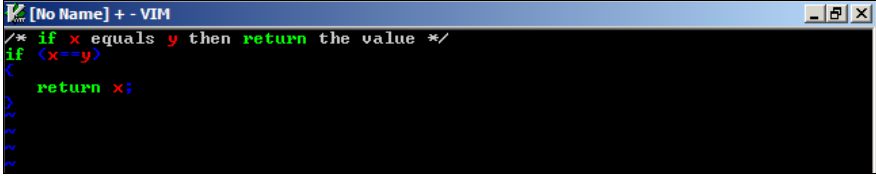
\includegraphics[scale=0.5]{./images/page142.png}
\end{center}

从上图中可以看到, 代码部分的高亮还不错, 可是注释语句却不令人满意. 这是因为我们
只是对单个单词进行匹配, 所以注释中的相同单词也会被匹配. 这种配置方法很难分辨出
代码与注释.
\marginpar{143}

那么, 我们可以从这个简单的例子里学习哪些东西呢? 那就是, 与高亮比起来, 更重要的
是要找到期望中的单词, 然后再给它们设置对应的颜色. 现在让我们增加一些上下文的信
息, 我们要把 \verb'/*' 与 \verb'*/' 之间的部分标记成注释, 然后再高亮其余的部
分. 代码部分被标记上颜色之后, 就不需要再上色了, 因此规则的顺序很重要. 具体的
配置代码是:
\begin{vimcode}
:syntax match myComments "/\*.*\*/"
:syntax keyword myVars x y
:syntax match mySymbols "[{}();=]"
:syntax keyword myKeywords if return
:highlight myVars ctermfg=red guifg=red
:highlight mySymbols ctermfg=blue guifg=blue
:highlight myKeywords ctermfg=green guifg=green
:highlight myComments ctermfg=yellow guifg=yellow
\end{vimcode}
最终的效果是:
\begin{center}
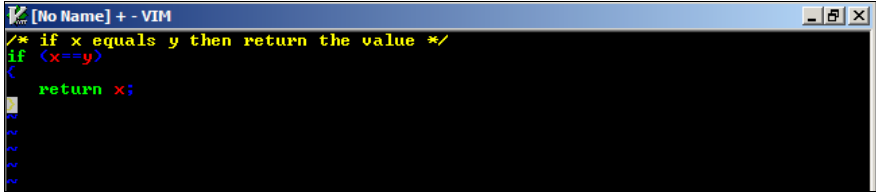
\includegraphics[scale=0.6]{./images/page143.png}
\end{center}

现在, 这段代码的高亮已经相当得体. 当然, 这只是一个小例子, 而且只用到了 Vim 语
法高亮的一小部分功能, 接下来, 我们将会介绍更多的内容.

\section{区域高亮}
\label{sec:syntax_regions}

在前面的例子中, 我们用的是选项 \texttt{match} 来选择注释语句. 在某些情况下,
我们很难创建一个适当的匹配语句, 这时候, 我们就需要用到其他一些更方便的做法.

在 Vim 中, 你可以选中一整个代码区, 然后再高亮它们, 为了选择一个代码区, 只需要
提供区域的开始与结束. 对于前面的例子, 如果使用区域高亮的话, 具体的命令是:
\begin{vimcode}
:syntax region myComments start=/\/\*/ end=/\*\//
\end{vimcode}
\marginpar{144}
有了这个命令, 很轻易就能匹配下面的任意一个注释块:
\begin{vimcode}
/* single line comment */
/*******************************
 *  multi line comments
 *******************************/
/* multi line comment
 */
\end{vimcode}

除了设置区域开始与结束, 选项 \texttt{region} 还可以做更多的事. 它还可以根据其
他语法规则来高亮区域内的某些代码. 我常做的一个操作是为函数注释设置几个关键词,
比如 \texttt{FIXME}, \texttt{OBSOLETE}, \texttt{TODO}, 等等, 这样, 我就可以把
代码写成:
\begin{vimcode}
/*  function: splitString()
 *  args    : string
 *  OBSOLETE
 */
function splitString(string) {
...
\end{vimcode}
剩下的工作, 就是创建一个关键词组:
\begin{vimcode}
:syntax keyword myKeywords OBSOLETE FIXME TODO
\end{vimcode}
现在, 我们需要修改命令 \texttt{region} 的设置, 以允许区域内包含其他语法元素,
修改后的命令是:
\begin{vimcode}
:syntax region myComments start=/\/\*/ end=\/\*\// contains=myKeywords
\end{vimcode}

如果需要在区域内包含多于一个语法组, 只需要把它们写成列表的形式 (列表元素之间
用逗号分开), 再写到 \texttt{contains} 的后面.

\begin{warning}
    只有当开始与结束都在同一行时, 你才能告诉 Vim 这个区域是正确的, 方法是在
    命令 \texttt{syntax} 中添加一行选项. 如果没有这个选项, Vim 会在遇到开始时
    就开始高亮代码, 遇到结束时 (或者是文件的末尾) 停止.
\end{warning}
\marginpar{145}

在某些情况下, 用户可以希望在一个区域中嵌套另一个区域, 对于这种情况, 用户必须
把这项需要显式地告诉 Vim, 方法是在区域命令的末尾加上选项 \texttt{contained}:
\begin{vimcode}
:syntax region myComments start=/\/\*/ end\/\*\// contains=myKeywords
contained
\end{vimcode}

在某些情况下, 一个代码块可以出现在代码中的任意一个位置, 当然, 用户不想针对每
一个代码块各写一个语法组, 这时候, 只需要把 \texttt{contains} 改成 \texttt{ALL}.

除了 \texttt{ALL}, 其他的关键词还包括:
\begin{itemize}
    \item \texttt{ALLBUT} 如果它是列表的第一项, 那么列表中的其余项目在区域中
        都不会被高亮显示
    \item \texttt{CONTAINED} 如果该项在列表中, 那么带有选项 \texttt{contained}
        的语法组就会在区域中被高亮显示
    \item \texttt{TOP} 如果该项在列表中, 那么除了带有选项 \texttt{contained}
        的语法组, 其他所有的语法都会被包含进来
\end{itemize}

有了上面的帮助, 用户就可以轻易地选择大范围的语法组, 而不用一个一个地把它们写下
来. 一个例子是选择除了 \texttt{myComments} 之外的所有语法组, 具体的命令是:
\begin{vimcode}
:syntax region myCodeblock start=/{/ end=/}/ contains=ALLBUT,myComments
\end{vimcode}

\begin{tips}
    如果用户知道某些语法组经常一起使用, 可以把它们放在一个簇 (cluster) 中:
    \texttt{:syntax cluster myCluster
    contains=myKeywords,mySymbols,myConditions}. 引用一个簇时可以在名字前加
    \verb'@': \texttt{:syntax region myComments start=/\/\*/ end=/\*\//
        contains=@myCluster}.
\end{tips}

现在, 用户只需要把所有的配置命令都写到一个文件中, 再把这个文件放到
\texttt{VIMHOME} 的 \texttt{syntax} 子目录中. 文件的后缀名是 \texttt{.vim},
前缀名是文件所对应的编程语言源代码文件的后缀名, 比如 C 语言源代码文件的后缀名
是 \texttt{.c}, 那么它的语法文件就是 \texttt{c.vim}.

在前面的例子中, 所有语法级的名字都以 \texttt{my} 开始, 这是因为它所对应的编程
语言是 \texttt{my} (当然, 只是假设性的). 如果是 C 语言, 那么比较好的做法是
语法组的名字以 \texttt{c} 开始, 比如 \texttt{cKeywords}, \texttt{cConditions},
\texttt{cSymbols}, 等等).

继续前面的例子, 我们刚才说到 \texttt{my} 语法文件所对应的编程语言源代码文件
的后缀名是 \texttt{.my}, 为了简便起见, 我希望 Vim 把我的文件识别成文件类型
\texttt{my}.
\marginpar{146}

如果 Vim 无法识别用户正在编辑的文件, 那么就需要注册它们. 方法是在
\texttt{VIMHOME} 目录下的 \texttt{filetype.vim} 中添加几行. 如果该文件不存在,
可以手工创建. 对我的编程语言来说, 需要添加以下几行:
\begin{vimcode}
augroup filetypedetect
autocmd BufNewFile,BufRead *.my setfiletype my
augroup END
\end{vimcode}
上面的代码告诉 Vim 把两行 \texttt{augroup} 之间的所有内容都添加给自动命令组
\texttt{filetypedetect}. 这个命令组用于确定文件所拥有的文件类型.

在我们的例子中, 命令的功能是无论何时打开一个后缀为 \texttt{.my} 的文件, 就把
它的文件类型设置成 \texttt{my}. 如果用户还想区别其他文件类型, 还可以在两行
\texttt{augroup} 之间添加其他 \texttt{autocmd}.

注意, 如果 Vim 检查到我们正在编辑的文件的文件类型是 \texttt{my}, 它就会自动
查找匹配的语法文件, 它会在目录 \texttt{VIMHOME/syntax/} 内查找以文件类型名开始
的语法文件, 在这里就是 \texttt{my.vim}.

% TODO
% This is all you need to get started on creating your own syntax files that
% Vim can automatically load whenever you open one of your files.

\begin{warning}
    学习编写语法文件的最佳方法是阅读别人写的语法文件. 安装 Vim 后, 就已经安装
    了大量的语法文件, 涵盖了几乎所有常见的文件类型, 用户可以以它们为基础, 从
    面写出自己的语法文件.
\end{warning}

另一方面, 如果用户想要在已存在的语法文件中添加额外的识别, 有两种方法可以做到.
其中一种是找到那个文件, 然后添加自己的内容, 另外一种更好的办法是使用 Vim 的后
处理功能, 该功能可以覆盖 Vim 已经加载的脚本或语法. 第二种办法可以做到无论系统
上的脚本怎么更新, 都不用改动自己的部分, 因为它们已经和脚本隔离开了.

使用后处理器的秘诀是脚本文件的存放位置. 在用户的 \texttt{VIMHOME} 目录下, 有一
个子目录 \texttt{after} (如果不存在, 则手工创建). 无论 Vim 在何时查找脚本, 语
法文件, 或配色方案, 它都会在 \texttt{after} 子目录内查找相同的文件. 比如说, 如
果 Vim 找到了 \texttt{VIMHOME/syntax/c.vim}, 它就会接着查找
\texttt{VIMHOME/after/syntax/c.vim}, 看看是否有需要覆盖的地方. 这种情况同样
适用于从下面这些目录找到的脚本:
\marginpar{147}
\begin{itemize}
    \item \texttt{plugin}
    \item \texttt{ftplugin}
    \item \texttt{indent}
    \item \texttt{autoload}
    \item \texttt{syntax}
    \item \texttt{colors}
\end{itemize}
只要用户需要某个文件, 就可以把上面的任意一个目录放到 \texttt{after} 目录下,
如果 Vim 找到了文件, 就会使用它.

\subsection{配色方案与语法高亮}
\label{subsec:color_scheme_and_syntax_coloring}

在前面的例子中, 我们通过命令 \texttt{:syntax} 添加了用户自己的高亮色彩组. 这
使得用户对配色具有了完全的控制权, 但同时也限制了颜色的种类. 因此, 在其他地方
可能就不能使用这些颜色\footnote{Hence, it might not follow the colors defined
by the color scheme you use in the rest of Vim}.

一个更好的办法是使用 Vim 已经定义好了的色彩组, 这就把色彩定义与语法高亮分成了
两个部分. 通过这种方法, 无论在何时修改了配色方案, 语法高亮都会自动地更新.

下面的命令可以列出所有已经定义了的颜色:
\begin{vimcode}
:highlight
\end{vimcode}

\begin{warning}
    或者, 你还可以看一下配色方案文件, 这些文件存放在 \texttt{VIMHOME} 的
    \texttt{color} 目录下.
\end{warning}

\section{使用脚本}
\label{sec:using_scripts}

每个人都会有一些特定的编辑器需求, 其中有些需求比较简单, 比如按键绑定, 而有一些
则比较复杂, 当然, Vim 不可能满足每个人的需要, 所以它提供了脚本供程序员扩展
Vim.
\marginpar{148}

但是如果用户不是个程序员, 或者没有时间自己开发脚本, 那又该怎么办呢? 这当然不是
个问题, Vim 是免费发布的, 因此有很多用户同样免费发布自己开发的脚本. 他们中的许
多人会把自己的脚本放到 \url{http://www.vim.org} 上供人免费下载, 其他用户很容易
就可以搜索到自己想要的脚本.

\subsection{脚本类型}
\label{subsec:script_types}

在 Vim 官网可以找到大量的脚本, 它们的功能各异, 有的很简单 (比如插入日期), 有的
则比较复杂 (比如 IDE 编程环境), 但是实际上, Vim 只能识别某几种定义了的脚本类型
组.

如果我们认真查看一下脚本类型, 就会发现它们可以分为两组, 第一组是全局插入组, 该
组包含的脚本会在 Vim 启动时, 或者是在用户执行某些特定的函数调用时补始化. 这种
脚本的典型例子包括为 Gvim 添加菜单, 为已经定义了的函数添加功能, 又或者是根据用
户的需要修改某些特性.

第二组是文件类型插件组. 该组包含的脚本和某个 (或某些) 特定的文件类型相关联, 只
有当相应类型的文件被打开或创建时, 才会加载脚本. 组内脚本的功能可以是为某个特定
的文件类型添加特性, 还可以是某些特定的工具. 比如, 为某种编程语言的编译操作定义
一个快捷键, 或者是在程序员编写的每一个函数上方添加一段注释. 组内的脚本还包括语
法高亮, 虽然和其他脚本相比, 语法高亮脚本的安装位置不太一样.

\subsection{安装脚本}
\label{subsec:installing_scripts}

下载脚本后, 它们的格式通常是下面三种之一:
\begin{itemize}
    \item 一个单一的 \texttt{.vim} 文件
    \item 一个压缩文件 (通常是 Zip 格式), 里面包含了一个或多个 \texttt{.vim}
        文件, 以及文档
    \item Vimball 格式, 一种 Vim 脚本安装文件
\end{itemize}

如果待安装的脚本仅仅是一个单一的脚本文件, 安装的方法是把它复制到
\texttt{VIMHOME/plugin} 目录下, 如果是和某种文件类型相关的脚本, 就复制到
\texttt{VIMHOME/ftplugin}.
\marginpar{149}
如果用户使用的是多用户操作系统, 只需要把它们安装在 Vim 安装目录 (而非
\texttt{VIMHOME}) 下面的同名子目录中, 就可以同时为所有的用户提供服务.

如果脚本被打包成压缩文件, 其安装方法就很难说清楚. 典型的安装方法是把压缩文件
复制到 \texttt{VIMHOME}, 然后再解压. 解压后, 压缩包中的文件会自动存放到对应的
目录内. 通常在压缩文件中都有一个 \texttt{README} 或 \texttt{INSTALL} 文件, 它
详细介绍了脚本的安装方法.

\begin{warning}
    如果脚本是在 \url{http://www.vim.org} 上找到的, 那就同时也能找到脚本的安
    装方法.
\end{warning}

最后一种格式需要通过 Vimball 安装, Vimball 是为 7 及以上版本的 Vim 而开发的.
Vim 接收若干个文件, 然后把它们组合在一个单一的 Vim 脚本归档文件, 文件的后缀名
是 \texttt{.vba}, 意思是 Vimball.

在开始使用 Vimball 之前, 得先安装 Vimball 脚本, 这个脚本用于读取与安装 Vimball
文件. 和其他脚本一样, 用户可以到 Vim 官网下载到该脚本.

\begin{warning}
    在 \url{http://www.vim.org/scripts/script.php?script_id=1502} 上可以下载
    到最新版的 Vimball.
\end{warning}

安装完 Vimball 脚本后, 就可以用它来安装其他 Vim 脚本.

假设用户现在有一个名为 \texttt{myscript.vba} 的 Vimball 文件, 为了安装它, 先
在 Vim 中打开该文件, 打开文件后, Vim 就会告诉用户如何安装
\texttt{myscript.vba}. 安装的方法通常是执行下面的命令:
\begin{vimcode}
:source %
\end{vimcode}
命令会把脚本安装到从选项 \texttt{runtimepath} 中找到的第一个目录内. 如果想修改
安装目录, 就把上面的命令换成:
\begin{vimcode}
:UseVimball PATH
\end{vimcode}
\marginpar{150}
你需要把 \texttt{PATH} 替换成脚本的安装路径. 需要注意的是, 有些脚本只能安装在
特定的目录下, 否则的话, 脚本就不能正常工作.

有时候, 用户可能想在安装之前查看一下 Vimball 中包含的文件. Vim 提供了一个这样
命令, 使用方法是在打开 Vimball 之后, 执行:
\begin{vimcode}
:VimballList
\end{vimcode}

查看后, 如果没什么问题, 就可以用 \texttt{:source} 或 \texttt{:UseVimball}
安装.

\subsection{卸载脚本}
\label{subsec:uninstalling_scripts}

通常来说, 不存在用于卸载脚本的自动化方法, 用户必须手动地把文件删除掉. 不过
Vimball 含有删除机制.

如果用户记得安装时所用的 Vimball 文件名, 就可以通过它来卸载脚本. 卸载 Vimball
的命令是:
\begin{vimcode}
:RmVimball VIMBALLNAME
\end{vimcode}
把 \texttt{VIMBALLNAME} 替换成安装脚本时所用的 Vimball 文件名. 如果脚本不是
安装有默认路径下 (通过 \texttt{:UseVimball} 命令), 就在命令的末尾加上安装路径:
\begin{vimcode}
:RmVimball VIMBALLNAME PATH
\end{vimcode}

为了把 Vimball 与将要删除的文件关联起来, 脚本会在 \texttt{VIMHOME} 下创建一个
名为 \texttt{.VimballRecord} 的文件. 注意, 如果你把这个文件删除了, 就不能卸载
之前所有的, 通过 Vimball 安装的脚本 (当然, 还可以通过手工删除来卸载).

\section{脚本开发}
\label{sec:script_development}

在使用 Vim 的过程中难免会遇到这样的情况: 自己想要的功能, Vim 却不提供. 所以现
在正好就是学习 Vim 脚本开发的好时机.

不过, 在开始前得先考虑几个问题.
\marginpar{151}
首先, 你必须确定你所想要的功能其他人还没有为此写过脚本 --- 干嘛要自己造轮子呢?
如果已经有人写了一个脚本, 而这个脚本的功能与你的非常接近, 那干嘛不直接修改他
的脚本, 从面扩展它的功能, 使得它既能服务于你, 又能服务于他人? 这种开发方法可
以缩短时间, 同时还可以避免类似脚本的泛滥.

如果你找不到满意的脚本, 那就得自己开发. 对于这些情况, 首先要考虑当脚本开发完成
后, 是否会发布它. Bram Moolenaar 将 Vim 免费发布, 很多脚本开发人员也是这么做
的, 所以笔者也希望你发扬分享的精神.

\begin{warning}
    关于开源许可证的更多信息, 登陆 \url{http://www.opensource.org/}.
\end{warning}

如果你决定分享你的脚本, 那你最好早早地就考虑到 Vim 可以运行在多种不同的平台上,
所以你的脚本最好也能够在这些平台上运行, 这意味着:
\begin{itemize}
    \item 不能期望某些外部工具是可用的
    \item 不能期望某些外部工具已经安装了, 即使你的确安装了它们
    \item 你必须记住, 在不同的平台上, 文件系统也有所不同
    \item 你必须记住某些功能只能在某些平台上使用
    \item 尽量使得各个特性是可配置的, 因为其他人可能并不喜欢它原来的样子
\end{itemize}

把这些记在心里后, 接下来就可以学习开发 Vim 脚本, 现在, 先让我们来看一些实际
的例子.

\subsection{脚本开发基础}
\label{subsec:script_writing_basics}

在接下来的几节, 我们将会介绍一些基本的类型与结构, 知道这些, 是开发出好脚本的
前提.

如果用户是一名程序员, 那就会对 Vim 的脚本语言感到很熟悉, 因为它的结构与其他
编程语言是类似的.
\marginpar{152}

\subsubsection{类型}
\label{subsubsec:types}

简单来说, Vim 只有两种类型的数据 --- 字符串与数值. 之所以是简单来说, 是因为
这两种类型还包含了其他的子类型. 一个数值可以有三种表示方法:
\begin{itemize}
    \item 十进制: 1, 2, 3, 100 等
    \item 十六进制: 0x01, 0x02, 0x03, 0xa0, 0x64 等
    \item 八进制: 01, 02, 03, 012, 0144 等
\end{itemize}

在表示十六进制与八进制数时, 需要分别在数的前面加外 \texttt{0x} 与 \texttt{0}.
Vim 可以方便地对数字进行运算, 即使数字间的进制不太相同, 比如, 可以计算下面的
表达式:
\begin{vimcode}
:echo 10 + 0x0A + 012
\end{vimcode}
运算结果是 \texttt{30}.

Vim 中的字符串用一对单引号或双引号括起来, 比如:
\begin{vimcode}
:echo "this is a string"
:echo 'this is a string'
\end{vimcode}

如果想在字符串中表示用于括住字符串的字符 (单引号或双引号), 就用反斜杆转义:
\begin{vimcode}
:echo "this is a string with a \" double quotes"
:echo 'the double quote " does not need escaping here'
\end{vimcode}

使用单引号还是双引号取决于具体的场景.

在单引号括住的字符串中, 字符串将会按照字面显示, 也被称为字面字符串. 这就意味着
在单引号括住的字符串中不能使用特殊的转义字符.

比如, 下面的字符串可以按照预想中的方式 (分成两行显示) 输出:
\begin{vimcode}
:echo "string with\n two lines"
\end{vimcode}
但这个就不可以:
\begin{vimcode}
:echo 'string with\n two lines'
\end{vimcode}
\marginpar{153}

除了换行符 \verb'\n', 其他的转义字符序列还包括:
\begin{tabular}{ll}
   \hline \\
   \verb'\n'    & 换行符 \\
   \verb'\r'    & 回车符 \\
   \verb'\t'    & 制表符 \\
   \verb'\123'  & 该八进制数所表示的字符 \\
   \verb'\x123' & 该十六进制数所表示的字符 \\
   \verb'\u'    & 最多 4 个十六进制数所表示的字符 \\
   \verb'\f'    & 换页 \\
   \verb'\e'    & 转码 \\
   \verb'\b'    & 退格 \\
   \hline
\end{tabular}

除了这些转义字符序列, 还可以插入其他 Vim 可识别的按键缩写, 比如 \texttt{<CR>},
与 \texttt{<ESC>}, 但是得在前面加上反斜杆 --- \verb'\<CR>', 甚至还可以插入其他
快捷键缩写, 比如 \texttt{<C-W>}, 但同样得加反斜杆.

\subsubsection{变量}
\label{subsubsec:variables}

Vim 有 5 种类型的变量 (虽然定义的方式是相同的), 使用方法也大不相同. 这 5 种类
型是:
\begin{itemize}
    \item 字符串: \texttt{"this is a string"} 就是一个简单的字符串
    \item 数值: 比如 \texttt{123} 或 \texttt{0x123}
    \item 线性表: 含有多个条目的有序序列 (或有序数组)
    \item 字典: 一个无序的关联数组, 保存有\ 键-值\ 对
    \item 函数引用: 指向一个函数的引用
\end{itemize}

变量的名字可以包含字母, 数字与下划线, 但不能以数字开始.

\begin{warning}
    尽量使用有意义的名字, 始终记住可能会有其他人阅读你的代码. 为了避免自己的
    变量名与别人的变量名混淆, 可以让自己的变量名以某个特殊的名字开始, 比如
    自己姓名的首字母缩写: \texttt{KSmyvariable}. 如果有多个程序员在开发同一
    套脚本, 那还可以用脚本文件名的缩写, 比如 Vim 排序脚本中的变量名可以是
    \texttt{VSmyvariable} 或 \texttt{VSSmyvariable}.
\end{warning}
\marginpar{154}

所有类型的变量都是通过命令 \texttt{:let} 定义:
\begin{vimcode}
:let myvar = VALUE
\end{vimcode}
命令中的 \texttt{VALUE} 取决于变量的具体类型. 对于字符串与数字, 定义的方式与
前面讲过的相同, 比如:
\begin{vimcode}
:let mystringvar = "a string"
:let mynumbervar = 123
\end{vimcode}
处理字符串与数值类型的变量时, 根据具体的使用方式, 这两种类型可以互相转换, 这
意味着即使执行了:
\begin{vimcode}
:let mystringvar="123"
\end{vimcode}
也可以使用:
\begin{vimcode}
:let mynumbervar=mystringvar-23
\end{vimcode}
在算术表达式中, \texttt{mystringvar} 会自动转换成数值类型.
\begin{warning}
    可以通过加 0, 从而把一个字符串强制转换成数值, 比如 \texttt{:let
    mynumber=mystringvar+0}. 为了把一个数值强制转换成字符串, 可以使用函数
    \texttt{string()}: \texttt{:let mystring=string(mynumber)}.
\end{warning}

这种自动类型转换对线性表与字典不适用, 因为它们包含的值可能一点也不相同. 下面
的表格汇总了类型转换的各种情况:
\begin{center}
    \begin{tabular}{ll}
        \hline \\
        输入类型 & 结果类型 \\
        \hline \\
        \texttt{"hello" . "world"}  & \texttt{"hello world"} (字符串) \\
        \texttt{"number" .123}  & \texttt{"number 123"}(字符串) \\
        \texttt{"123" + 10} & \texttt{133} (数字) \\
        \texttt{"123" - 10 . "hits"} & \texttt{"113 hits"} (字符串) \\
        \texttt{"123" - 10 + "hits"} & \texttt{113} (数值) \\
        \hline
    \end{tabular}
\end{center}

定义线性表的方式是将表内的各个值用逗号分开, 外面再包围一对中括号:
\begin{vimcode}
:let mylistvar1 = [1,2,"three",0x04,myfivevar]
\end{vimcode}
线性表的元素还可以是一个线性表:
\begin{vimcode}
    :let mylistvar2 = [[1,2,3],["four","five","six"]]
\end{vimcode}
\marginpar{155}

可以看到, 上面定义的线性表包含了字符串, 数值, 和线性表. 因此线性表可以作为存
放不同类型变量的容器.

稍后, 我们将会介绍如何使用线性表中的变量, 以及如何与其他线性表一起工作.

创建一个字典变量的命令是:
\begin{vimcode}
:let mydictvar1 = {1: "one", 2: "two", 3: "three"}
\end{vimcode}
命令创建了包含三个项目的字典变量, 项目的键是数值, 值是字符串.

不管把键写成数值, 还是字符串, Vim 都会把它们转换成字符串, 所以上面的命令会把
键值对定义成 \texttt{1:one}.

字典中还可以包含其他字典, 比如:
\begin{vimcode}
:let mydictvar2 = {1: "one", 2: "two", "tens":{0: "ten", 1: "eleven"}}
\end{vimcode}
可以看到, 键不需要遵守特别的顺序, 也不一定非得是数值类型 (比如例子中的
\texttt{"tens"}).

稍后, 我们将会介绍如何访问字典中的值, 以及字典与线性表之间如何互相转换.

最后一种变量类型是函数引用, 这种类型的变量包含了指向某个函数的引用, 和其他类
型的变量相比, 其不同点是它是可执行的. 定义函数引用的命令是:
\begin{vimcode}
:let Myfuncrefvar = function("Myfunction")
\end{vimcode}
命令把变量 \texttt{Myfuncrefvar} 绑定到函数 \texttt{Myfunction}. 需要注意的是,
变量名以大写字母开始, 这是因为所有的用户自定义函数的函数名都以大写字母开始,
因此作为函数执行的变量也要遵命这个规定.

在使用函数引用类型的变量时, 只需要在函数名的后面加上一对括号:
\begin{vimcode}
:echo Myfuncrefvar()
\end{vimcode}
除此之外, 还可以用:
\begin{vimcode}
:call Myfuncrefvar()
\end{vimcode}
\marginpar{156}

如果函数所绑定的函数需要输入参数, 那就把参数放到括号中, 就像
\texttt{Myfuncrefvar(arg1, arg2,..., argN)}.

变量可以拥有不同的作用域, 这意味着某些变量只能在函数内访问, 而有些变量可以在
任意一个地方被访问到.

脚本开发人员需要把变量的作用域告诉给 Vim, 方法是在变量名的前面加上作用域指示
符.

如果在定义变量时没有定义作用域, 那就是全局的, 如果变量是在函数内定义的, 那么
作用域仅限于函数内部. 总共有以下 8 种作用域:
\begin{itemize}
    \item \texttt{v}: Vim 预定义的全局作用域
    \item \texttt{g}: 全局作用域
    \item \texttt{b}: 缓冲区作用域 --- 只在定义变量的缓冲内有效
    \item \texttt{t}: 标签页作用域 --- 只在定义变量的标签页内有效
    \item \texttt{w}: 窗口作用域 --- 只在当前窗口内有效
    \item \texttt{l}: 函数作用域 --- 只在定义它的函数内部有效
    \item \texttt{s}: 来源文件作用域 --- 只在通过命令 \texttt{:source} 加载的
        文件内有效
    \item \texttt{a}: 参数作用域 --- 专门用于函数的参数
\end{itemize}

\begin{warning}
    % TODO
    Did you know that comments in Vim scripts are created by having a quote as
    the first non-space character on the line: \texttt{" this is a comment}?
\end{warning}

下面的程序用到了几个不同的作用域:
\begin{vimcode}
let g:sum=0
function SumNumber(num1,num2)
    let l:sum = a:num1+a:num2
    "check if previous sum was lower than this
    if g:sum < l:sum
        let g:sum=l:sum
    endif
    return l:sum
endfunction
" test code, this will print 7 (value of l:sum)
echo SumNumbers(3,4)
" this should also print 7 (value of g:sum)
echo g:sum
\end{vimcode}
\marginpar{157}

虽然局部变量与全局变量的名字可以相同, 但是如果你已经知道某个全局变量的名字,
最好就不要再使用同名的局部变量.

\begin{warning}
    尽量使用具体的作用域. 这种方法可以避免全局变量被一些你无法控制的变量所
    污染.
\end{warning}

\subsubsection{条件}
\label{subsubsec:conditions}

开发 Vim 脚本时, 有时候在执行代码之间需要检查某个条件是否满足. 大多数现代
编程语言使用条件语句进行条件检查. Vim 同样也有这种语句, 它的格式是:
\begin{vimcode}
if condition
    code-to-execute-if-condition-is-met
endif
\end{vimcode}
如果 \texttt{condition} 的值为真, \texttt{if} 和 \texttt{endif} 之间的语句就
会执行, 否则就不执行.

那么, 在这个 \texttt{if} 结构中我们可以使用哪些条件? 主要有两种 --- 使用逻辑
运算符的语句, 与使用字符串运算符的语句. 现在来看一下这两种运算符如何使用. 其
总的形式都是:
\begin{vimcode}
value1 OPERATOR value2
\end{vimcode}
命令中的 \texttt{OPERATOR} 是用于比较 \texttt{value1} 与 \texttt{value2} 的运
算符. 比如:
\begin{vimcode}
value1 >= value2
\end{vimcode}
如果 \texttt{value1} 大于或等于 \texttt{value2} 则表达式为真. 这只是逻辑运算符
中的一种, 其他的逻辑运算符还有:
\begin{itemize}
    \item \texttt{val1 == val2}: 如果 \texttt{val1} 等于 \texttt{val2}, 则表达
        为真
    \item \texttt{val1 != val2}: 如果 \texttt{val1} 不等于 \texttt{val2}, 则
        表达为真
    \item \texttt{val1 > val2}: 如果 \texttt{val1} 大于 \texttt{val2}, 则
        表达为真
    \item \texttt{val1 < val2}: 如果 \texttt{val1} 小于 \texttt{val2}, 则
        表达为真
    \item \texttt{val1 >= val2}: 如果 \texttt{val1} 大于或等于 \texttt{val2},
        则表达为真
    \item \texttt{val1 <= val2}: 如果 \texttt{val1} 小于或等于 \texttt{val2},
        则表达为真
\end{itemize}
\marginpar{158}

这些运算符既可以用于数值类型, 也可以用于字符串类型, 因为 Vim 可以自动进行转
换. 如果是对字符串进行比较, 在比较时会逐字比较各个字母的 ASCII 码值. 例如
\texttt{"bbb" > "aaa"} 为真, 而 \texttt{"abc" > "abd"} 为假 (这是因为
\texttt{a} 的 ASCII 值比 \texttt{d} 小).

如果是对字符串进行处理, 还有更多的运算符可供选择. 如果用户想查看某个字符串是
含有特定的子字符串或字符, 则可以使用部分匹配运算符, 使用方式是:
\begin{itemize}
    \item \texttt{str1 =~ str2}: 如果 \texttt{str1} 包含 \texttt{str2}, 或
        \texttt{str1} 与 \texttt{str2} 相同, 则为真
    \item \texttt{str1 !~ str2}: 如果 \texttt{str1} 不包含 \texttt{str2}, 并且
        \texttt{str1} 与 \texttt{str2} 不相同, 则为真
\end{itemize}

使用这两个运算符时, \texttt{str2} 通常是一个模式, 并且可以使用 Vim 的正则表达
式 (见 \texttt{:help regexp}). 这就意味着不仅仅可以进行简单的匹配, 还可以是非
常复杂高级的匹配.

所有的这些条件运算符都可以用于 \texttt{if} 语句内, 稍后你将会看到, 它们还可以
用在其他地方.

现在来看几个条件表达式的具体使用示例.

在某些情况下, 用户可能希望某块代码只在某个条件满足时才执行, 当条件不满足时执行
另一块代码. 这种情况下可以使用两个 \texttt{if} 条件 ---  一个用于检查条件是否
为真, 另一个用于检查条件是否为假. 不过, 还有另一种方法.

另一种方法是使用 \texttt{if-else-endif} 语句, 它的使用方法是:
\begin{vimcode}
if condition
    code-to-execute-if-condition-is-true
else
    code-to-execute-if-condition-is-NOT-true
endif
\end{vimcode}
\marginpar{159}

另一种情况是需要检查多个条件, 而且只有其中一个条件会满足, 代码的形式是:
\begin{vimcode}
if condition1
    code-to-execute-if-condition1-is-true
else
    if condition2
        code-to-execute-if-condition2-is-true
    endif
endif
\end{vimcode}

可以看到, \texttt{condition1} 与 \texttt{condition2} 中只有一个的值可以为真,
并且两个都可以为假. 但是这样的代码是成簇的, 额外的 \texttt{endif} 如果放的位
置不对, 会导致错误的 \texttt{if} 结构.

一个更好的方式是使用 \texttt{if-elseif-else} 结构:
\begin{vimcode}
if condition1
    code-to-execute-if-condition1-is-true
elseif condition2
    code-to-execute-if-condition2-is-true
endif
\end{vimcode}

这段代码所做的工作与前一个的相同, 但是它的可读性更高. \texttt{elseif} 出现的
次数可以多于一次, 这就意味着可以在同一个结构中判断多个条件, 而不用担心会出现
什么问题.

稍后, 我们将会介绍如何在循环结构中使用条件判断.

\subsubsection{使用线性表与字典}
\label{subsubsec:working_with_lists_and_dictionaries}

在之前的内容中, 我们已经介绍了如何创建线性表与字典, 现在讨论如何访问这两个结
绝中的数据.

如果用户已经有了一个线性表变量, 并且想要访问其中的某个变量, 访问的方法是在线
性变量的名字后面加上一对方括号, 并在括号内填上所要访问的值在线性表中的索引.
索引是表项在线性表中的存放位置, 从 \texttt{0} 开始. 假设我们想要访问下面线性
表中的元素 \texttt{"three"}:
\begin{vimcode}
:let mylistvar1 = [1,2,"three",0x04,myfivevar]
\end{vimcode}
\marginpar{160}
\texttt{"three"} 的索引是 2, 所以我们可以这样访问它:
\begin{vimcode}
:echo mylistvar[2]
\end{vimcode}
如果线性表中还有线性表, 比如 \texttt{mylistvar2}:
\begin{vimcode}
    :let mylistvar2 = [[1,2,3],["four","five","six"]]
\end{vimcode}
如果想要访问 \texttt{"four"} 所在的元素, 我们需要访问里面那个线性表的索引 0,
与外面那个线性表的索引 1:
\begin{vimcode}
:echo mylistvar2[1][0]
\end{vimcode}

在线性表中还可以使用负的索引值. 如果索引值是负的, 那个这个索引就是相对于表的
末尾, 而不是开头. 所以, 访问 \texttt{"four"} 的另一种形式是:
\begin{vimcode}
:echo mylistvar2[-1][-3]
\end{vimcode}
因为 -0 与 0 是相同的, 所以最后一项的索引是 -1.

\begin{warning}
    如果试图访问一个不存在的元素, Vim 就会返回一个错误. 为了避免返回错误信息,
    可以用 \texttt{get()} 来获取元素: \texttt{:echo get(mylistvar1, 2)}, 其中
    \texttt{2} 是试图访问的元素的索引.
\end{warning}

如果想要往一个已存在的线性表中添加一个新元素, 有很多种方法都可以做到. 最简单的
方式是用函数 \texttt{add()}, 它的一个使用示例是:
\begin{vimcode}
:let mylistvar3 = [1,2,3,4]
:call add(mylistvar3, 5)
:echo mylistvar3
\end{vimcode}
上面的命令在 \texttt{mylistvar3} 添加一个新元素 \texttt{5}, 然后打印整个线性
表. 添加元素的另一种方法是使用 Vim 的拼接功能. 运算符 \texttt{+} 可以用于拼接
两个线性表, 它的一个使用示例是:
\begin{vimcode}
:let mylistvar4 = [1,2,3,4]
:let mylistvar4 = mylistvar4 + [5,6,7,8]
:echo mylistvar4
\end{vimcode}
上面的命令先是创建一个具有 4 个元素的线性表, 然后再拼接上一个新的线性表, 再把
拼接后的线性表赋给自己. 最终, 线性表中将含有 8 个元素.
\marginpar{161}

\begin{warning}
    在拼接两个线性表时, 还有一个更方便的运算符: \texttt{+=}. 这个运算符可以把
    右手边的线性表拼接到左手边的线性表上, 比如: \texttt{:let mylistvar4 +=
    [5,6,7,8,]}
\end{warning}

如果待拼接的线性表只含有一个元素, 那么它的效果与添加一个新元素是相同的.

除了运算符 \texttt{+}, 还可以用函数 \texttt{extend()} 来完成拼接. 它的一个使
用例子是:
\begin{vimcode}
:let mylistvar5 = [1,2,3,4]
:call extend(mylistvar5, [5,6,7,8])
:echo mylistvar5
\end{vimcode}
注意, \texttt{add()} 与 \texttt{extend()} 之间有很大的不同. 在上面的例子中如果
把 \texttt{extend()} 换成 \texttt{add()}, 那么最终的结果是把一个线性表添加到
另一个线性表中, 相当于:
\begin{vimcode}
:let mylistvar5 = [1,2,3,4,[5,6,7,8]]
\end{vimcode}
这个线性表只有 5 个元素, 面且最后一个元素是一个含有 4 个元素的线性表.

移除元素的方法与添加元素的方法类似, 只不过要把 \texttt{add()} 换成
\texttt{remove()}, 比如:
\begin{vimcode}
:call remove(mylistvar5, 3)
\end{vimcode}
这个命令从 \texttt{mylistvar5} 中移除索引为 \texttt{3} 的元素.

现在开始介绍如何访问与修改字典变量. 在前面我们已经介绍过创建一个字典变量的命令
类似于:
\begin{vimcode}
:let mydictvar1 = {1: "one", 2: "two", 3: "three"}
\end{vimcode}

访问字典变量的方式与线性表非常类似. 假如我们想访问 \texttt{"two"}, 那就得在字
典变量的后面加个 \texttt{[]}, 并在括号内填上它的键值, 就像:
\begin{vimcode}
:echo mydictvar1[2]
\end{vimcode}
\marginpar{162}

看起来和访问线性表差不多, 但是如果把键值改成字符串, 那就不一样了:
\begin{vimcode}
:let mydictvar4 = {'banana': 'yellow', 'apple': 'green'}
\end{vimcode}
现在, 我们想要访问苹果的颜色:
\begin{vimcode}
:echo mydictvar4['apple']
\end{vimcode}
上面的命令会在屏幕打印出 \texttt{'green'}. 如果键值仅由 ASCII 字母, 数字, 与
下划线组成, 则还可以用:
\begin{vimcode}
:echo mydictvar4.apple
\end{vimcode}
键值的第一个字符必须是 ASCII 字母.

线性表中的元素是有序的, 并且含有索引, 相比之下, 字典是无序的, \mbox{键}-值
对中的键用于获取对应的值.

修改字典中的某个值的命令是:
\begin{vimcode}
:let mydictvar4['apple'] = 'red'
\end{vimcode}
往字典变量中添加新元素的命令和上面的相同, 唯一需要注意的地方是所使用的键必须是
变量中未出现过的.

用户可以在字典变量上附加一个函数, 使用该函数可以对字典变量中的元素进行一些操
作, 接下来我们将通过一个例子来说明.

比如说, 我们想要达到这样一个功能: 接收一个数值, 把数值中每一个数位上的数字转
换成对应的英文拼写形式. 假设完成这个转换过程的函数是 \texttt{convert}, 而它
所附加的字典变量是:
\begin{vimcode}
:let mynumbers = {0:'zero',1:'one',2:'two',3:'three',4:'four',
                5:'five',6:'six',7:'seven',8:'eight',9:'nine'}
\end{vimcode}
函数是:
\begin{vimcode}
function mynumbers.convert(numb) dict
    return join(map(split(a:numb,'\zs'),'get(self, v:val,"unknown")'))
endfunction
\end{vimcode}
上面的函数代码中有两个地方需要注意.

第一个需要注意的地方是函数的定义方式与普通函数的定义方式相同, 除了函数名需要
包含字典变量的名字, 并且在函数参数的后面需要加上关键字 \texttt{dict}.
\marginpar{163}
这个关键词告诉 Vim 把该函数当成一个字典函数, 并对一个特殊的变量作操作 ---
\texttt{self}, 在这个例子中, 变量 \texttt{self} 指向函数所关联的字典变量.
这意味着我们可以通过 \texttt{self[1]} 来获取值 \texttt{"one"}, 以此类推. 函数
的实现由四个子函数组成:
\begin{itemize}
    \item \texttt{split}: 把存放在变量 \texttt{a:numb} 中的参数切分到一个匿名
        线性表中, 例如:
    \begin{vimcode}
    :let a = split("one two")
    :echo a;    " this prints "one"
    \end{vimcode}
\item \texttt{map}: 把一个给定的命令映射到线性表 (通过调用 \texttt{split}
    得到的线性表) 中的每一个元素上, 例如:
    \begin{vimcode}
    :let mylist = ["one", "two", "three"]
    :call map(mylist, "<" . v:val . ">")
    :echo mylist[0] " this prints <one>
    \end{vimcode}
\item \texttt{get}: 从 \texttt{self} 中取一个键值是 \texttt{v:val} (从
    \texttt{map} 中获取的值) 的元素, 例如:
    \begin{vimcode}
    :let mylist2 = ["one", "two", "three"]
    :echo get(mylist2, 2, "none") " prints three
    :echo get(mylist2, 3, "none") " prints "none"
    \end{vimcode}
\item \texttt{join}: 连接所有的, 由 \texttt{map}-\texttt{get} 返回的元素,
    例如:
    \begin{vimcode}
    :let mylist3 = ["one", "two", "three"]
    :let mystring = join(mylist3, "+")
    :echo mystring " prints one+two+three
    \end{vimcode}
\end{itemize}
更多的信息请参考 \texttt{:help split()}, \texttt{:help join()},
\texttt{:help map()}, \texttt{:help get()}.

说得更明白一点, 函数 \texttt{mynumbers.convert} 的功能是接收一个范围内的数字
(\texttt{a:numb}), 然后把它切分成单独的数字, 再把每个数字当成一个键去索引字典
(\texttt{mynumbers}, 或 \texttt{self}) 中对应的值, 把所有返回的值连接起来,
值与值之间用一个空格分开, 最后再返回这个字符串.

现在, 用户可以把自己的字典变量当成一个转换器, 把数值转换成对应的英文形式, 使
用方式是:
\begin{vimcode}
:echo mynumbers.convert(12345)
\end{vimcode}
\marginpar{164}
上面的命令将会打出 \texttt{"one two three four five"}, 正好就是 \texttt{12345}
的英文表示形式.  % TODO: This is a functionality that opens up a lot of new
% possibilities.

\subsubsection{循环}
\label{subsubsec:loops}

在处理线性表或字典类型的变量时, 经常需要遍历变量中的所有元素, 对于这种情况,
程序员通常会使用循环结构, Vim 同样也提供了这种结构.

Vim 提供了两种形式的循环:
\begin{itemize}
	\item \texttt{for} 循环
	\item \texttt{while} 循环
\end{itemize}
接下来, 我们将会介绍如何使用这两个循环.

\paragraph{\texttt{for} 循环}
\label{para:for_loops}

\texttt{for} 循环可以有多种构造方式, 其中最简单的一种是:
\begin{vimcode}
for var in ranges
	do-something
endfor
\end{vimcode}
在上面的形式中, 循环依次遍历每一个元素, 每次迭代都会更新变量 \texttt{myvar} 的
值, 一个例子是:
\begin{vimcode}
for myvar in range(1,10)
	echo myvar
endfor
\end{vimcode}
上面的命令使用了函数 \texttt{range()} 来生成从 1 到 10 的整数, 循环从 1 开始
遍历所有的数. 循环的每次迭代都会把变量 \texttt{myvar} 的值更新成当前从范围中
所取得的值. 循环结束后, 将会打印出 1 到 10 这十个数字.

虽然上面的命令并没有用到线性表, 但是很容易就可以把函数替换成线性表, 换成线性
表后的形式是:
\begin{vimcode}
for var in list
	do-something
endfor
\end{vimcode}
\marginpar{165}
上面的命令形式非常简单, 现在来看一个具体的使用例子:
\begin{vimcode}
let mylist = ['a','b','c','d','e','f','g','h','i','j','k']
for itemvar in mylist
    echo itemvar
endfor
\end{vimcode}
命令执行时, 会陆续打印从 \texttt{a} 到 \texttt{k} 的所有字母. 用 \texttt{for}
循环遍历线性表的代码都遵循上面的形式.

如果想要循环打印字典变量中的元素, 则需要多做一点工作, 这是因为字典变量的元素
与一个键关联, 而不是索引. 但是有一个函数可以帮助我们从字典变量中提取键, 然后
就可以像处理线性表那样, 遍历所有的键, 这个函数的名称是 \texttt{keys()}. 先
来看一下使用示例:
\begin{vimcode}
let mydict = {a:"apple", b:"banana", c:"citrus" }
for keyvar in keys(mydict)
    echo mydict[keyvar]
endfor
\end{vimcode}
在上面的例子中, 我们从字典变量 \texttt{mydict} 中获取到一个包含了所有键的线
性表, 然后遍历表中的每一个元素, 将元素的值放到变量 \texttt{keyvar} 中, 然后
再用 \texttt{keyvar} 从字典变量中获取对应的值.

因为字典变量中的各个元素是无序的, 所以上面的命令可能会打印出 \texttt{banana
citrus apple}. 有个函数可以对键进行排序, 从面得到有序的值, 这个函数是
\texttt{sort}:
\begin{vimcode}
let mydict = {a:"apple", b:"banana", c:"citrus" }
for keyvar in sort(keys(mydict))
    echo mydict[keyvar]
endfor
\end{vimcode}
使用 \texttt{sort} 的前提是键是可排序的, 这对上面的例子来说并不成问题:
\texttt{a} 排在 \texttt{b} 之前, 而 \texttt{b} 排序在 \texttt{c} 之前.

\begin{warning}
    \texttt{sort} 还可以第二个参数, 这个参数是一个函数名, 这就使得用户可以
    提供自己的排序函数. 更多的信息与示例请参考 \texttt{:help sort()}.
\end{warning}
\marginpar{166}
